% Tiempo frente a talla: un panel por metodo, en el mismo orden que la memoria (GGH, LWE, Ring-LWE).
% Para que se lea sin interpretar el eje logaritmico, cada punto lleva escrito su tiempo (debajo y a
% la derecha) y entre dos puntos seguidos se indica por cuanto se multiplica (encima de la linea).
% Datos: generar_datos.py y generar_datos_lwe.py (\CurvaGGH, \CurvaLWE, \FactoresLWE, ...).
\pgfplotsset{panel/.style={
  scale only axis,width=3.6cm,height=2.8cm,
  log ticks with fixed point,
  /pgf/number format/use comma,/pgf/number format/1000 sep={},
  grid=major,grid style={gray!20},
  title style={font=\small},
  tick label style={font=\small},label style={font=\small},
  nodes near coords,point meta=explicit symbolic,
  every node near coord/.append style={black,font=\footnotesize,anchor=north west,inner sep=1.5pt},
  enlarge y limits=0.25,clip=false}}
\tikzset{factor/.style={font=\footnotesize,anchor=south east,inner sep=1pt}}
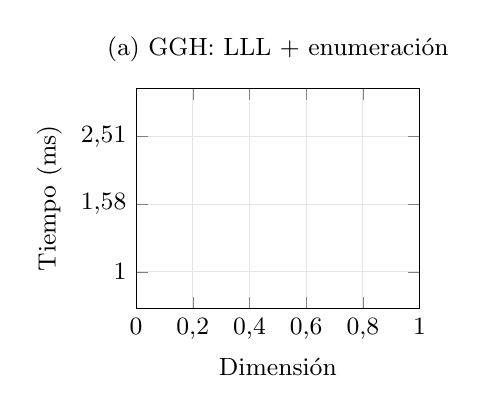
\begin{tikzpicture}
\begin{semilogyaxis}[panel,title={(a) GGH: LLL + enumeración},ylabel={Tiempo (ms)},
  xlabel={Dimensión},xmin=1,xmax=24,xtick={2,7,15},ytick={0.1,1,10}]
\addplot[black,mark=*,mark size=1.6pt,line width=0.7pt] coordinates {\CurvaGGH};
\end{semilogyaxis}
\end{tikzpicture}\hfill
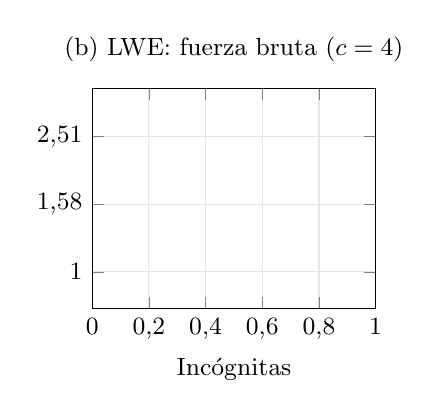
\begin{tikzpicture}
\begin{semilogyaxis}[panel,title={(b) LWE: fuerza bruta ($c=4$)},
  xlabel={Incógnitas},xmin=2.6,xmax=6,xtick={3,4,5},ytick={10,100,1000}]
\addplot[black,mark=*,mark size=1.6pt,line width=0.7pt] coordinates {\CurvaLWE};
\FactoresLWE
\end{semilogyaxis}
\end{tikzpicture}\hfill
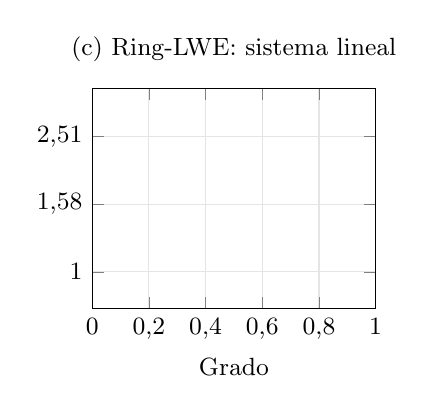
\begin{tikzpicture}
\begin{semilogyaxis}[panel,title={(c) Ring-LWE: sistema lineal},
  xlabel={Grado},xmin=8,xmax=100,xtick={16,32,64},ytick={10,100,1000}]
\addplot[black,mark=*,mark size=1.6pt,line width=0.7pt] coordinates {\CurvaRing};
\FactoresRing
\end{semilogyaxis}
\end{tikzpicture}
